\chapter{Ingeniería de software}
\label{sec:sftw}
Todo el desarrollo de este trabajo se ha realizado en Python. Python es un lenguaje de programación de alto nivel diseñado por Guido van Rossum y aparece en 1991. Este lenguaje está centrado en la legibilidad del código, siendo un lenguaje interpretado. \linebreak
Python también provee un gestor de paquetes llamado \textit{pip} que permite crear e instalar librerías externas, proporcionando así una mayor comodidad para hacer uso de librerías externas que lenguajes como C no tienen. \\
Uno de los mayores inconvenientes que tiene Python es que es un \textit{lenguaje interpretado} donde un interprete lee y ejecuta las instrucciones escritas en un \textit{script}, haciendo que el rendimiento sea menor que el de un programa que haya sido compilado.\\
\linebreak 
Además de hacer uso de este lenguaje, se ha usado \textbf{git} y \textbf{GitHub}.\\
\textbf{Git} es un Sistema de Control de Versiones de Software Libre diseñado por Linus Torvalds. Su propósito es registrar todos los cambios que se realizan sobre el código fuente.\\
\linebreak
\textbf{GitHub} es una plataforma que permite alojar proyectos software usando el Sistema de Control de Versiones \textbf{git}. Fue desarrollado por Chris Wanstrath, P. J. Hyett, Tom Preston-Werner y Scott Chacon usando Ruby on Rails en 2008.\\
\linebreak
Finalmente, para crear los diagramas que se verán en las secciones siguientes, se ha usado \textbf{PlantUML}. PlantUML es una herramienta de código abierto que permite crear diagramas a partir de archivos de texto, de forma similar a Latex. El autor es Arnaud Rosques y la primera versión de esta herramienta fue liberada en 2009.
\clearpage
\section{Horas de trabajo y presupuesto}
Para el desarrollo de este trabaja se ha dedicado de entre 8-9 horas semanales durante unos 9 meses, dando un total de unas $306$ horas en total. Si consideramos un valor de 15 euros por hora, este trabajo se pagaría por un total de $4590$\euro. 
\begin{figure}[H]
 	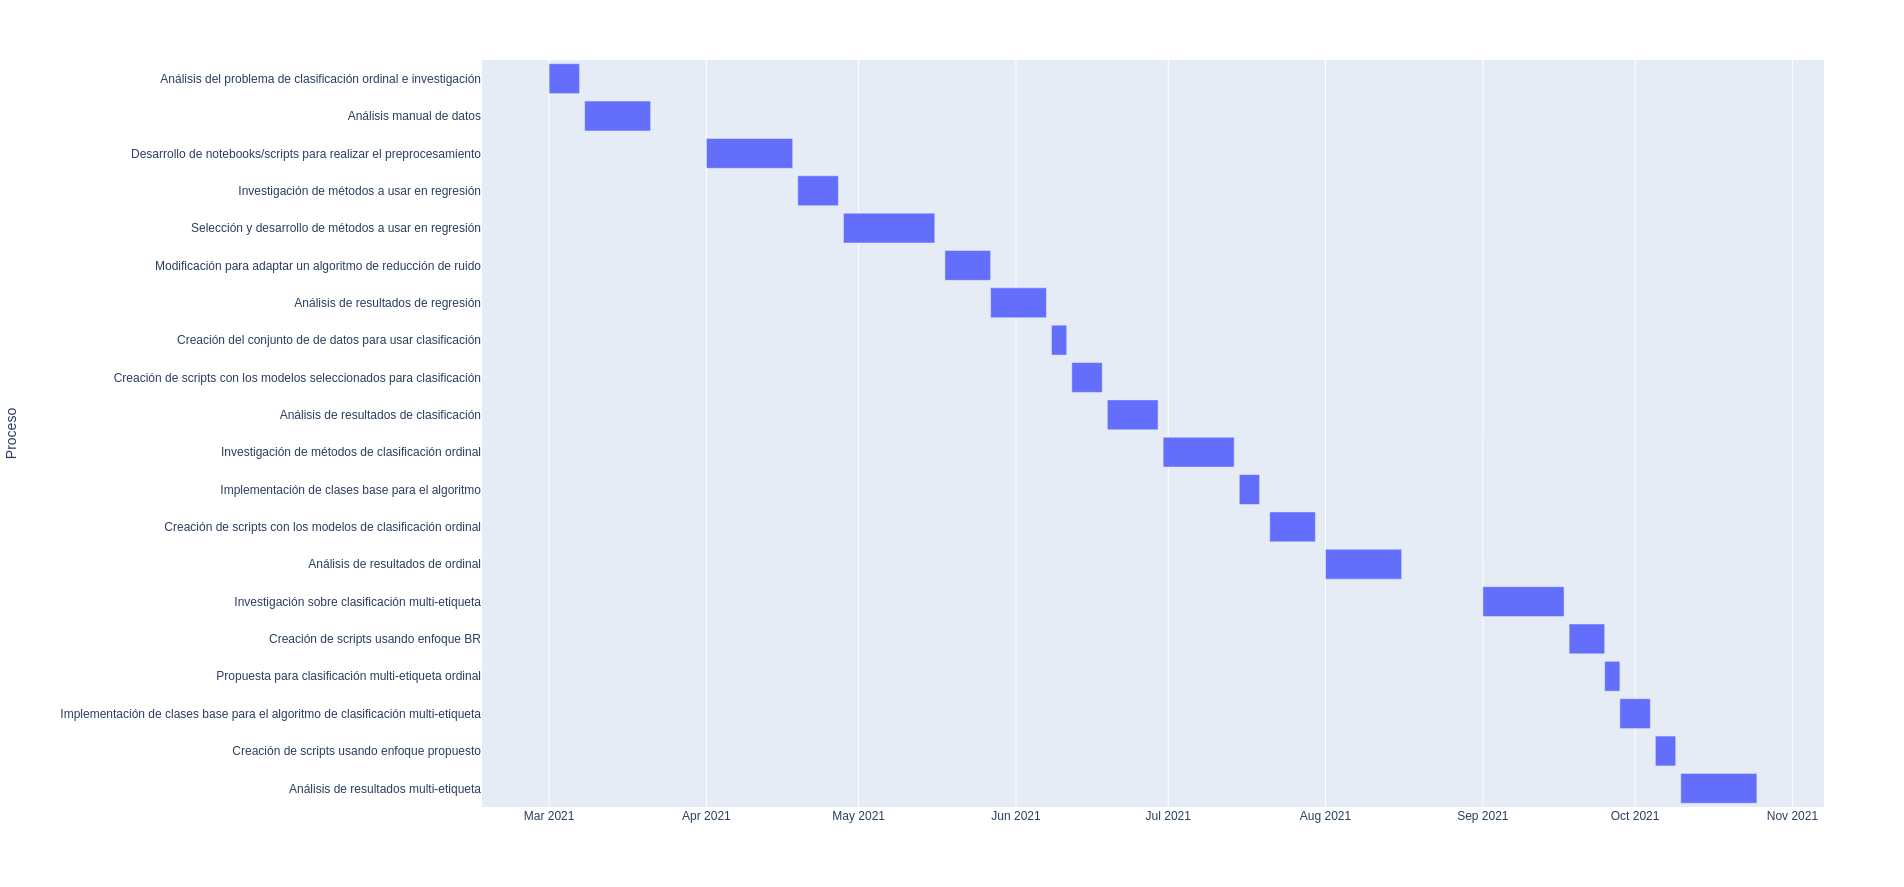
\includegraphics[scale=0.25]{gantt}
	\caption{Diagrama de Gantt}
	\label{fig:gantt}
\end{figure}
En la Figura \ref{fig:gantt} se muestra las horas dedicadas al desarrollo de este trabajo usando un Diagrama de Gantt. En el eje vertical aparecen las distintas fases del proyecto, y en el eje horizontal aparece una estimación de los días empleados para realizar el proyecto.\\
\linebreak
Todo el proyecto se ha realizado en un ordenador portátil HP-Omen 15 con las siguientes especificaciones: \textbf{CPU:} Ryzen 7 4800H, \textbf{RAM:} 16GB y \textbf{SSD:} 1TB y usando el sistema operativo Ubuntu 21:04.\\
Con un precio de alrededor 1000\euro, el importe total de este proyecto ascendería a unos $5590$\euro.\\
\linebreak
Todas estas estimaciones se han realizado sin tener en cuenta el proceso de obtención de datos, donde habría que tener en cuenta la realización de la encuesta, la toma de datos y transcripción a un formato digital. Esta información no ha sido compartida con nosotros, por lo que no podemos estimar cuanto tiempo y dinero se le sumaría al total que se ha mencionado antes.
\clearpage
\section{Biblioteca usadas}
Para realizar este trabajo, se ha hecho uso de una serie de \textbf{bibliotecas externas} que incrementan las capacidades ofrecidas por el lenguaje de manera nativa, ya que la gran mayoría de herramientas que han sido usadas no vienen instaladas por defecto.\\
A continuación, se listan las librerías usadas y una breve descripción de las herramientas/características que ofrecen:
\begin{itemize}
    \item \textbf{scikit-learn:} Es una biblioteca para aprendizaje automático que incluye una gran cantidad de algoritmos (SVM, árboles de decisión, Random Forest, etc) y distintas utilidades (métricas, validación cruzada, división de conjunto de entrenamiento y de test, etc). Es de software libre y está programada en C, C++ y Python.
    \item \textbf{Numpy}: Es una biblioteca que da soporte para crear vectores y matrices de grandes dimensiones junto con una colección de funciones para operar con estos tipos de datos. De nuevo, es una biblioteca de software libre y está escrita en Python, C y Fortran.
    \item \textbf{matplotlib}: Es una biblioteca para generar gráficos escrita en C++ y Python.
    \item \textbf{seaborn}: Es una biblioteca basada en \textit{matplotlib} que proporciona una interfaz de alto nivel para crear gráficos. Está escrita en Python.
    \item \textbf{pandas}: Es una biblioteca para la manipulación y análisis de datos.  Está escrita como una extensión de \textit{numpy}, siendo también software libre.
    \item \textbf{xgboost}: Biblioteca que proporciona una implementación para el algoritmo XGBoost.
\end{itemize}
Para facilitar la instalación de todas estas librerías de manera que no proporcionen conflictos, se ha optado por usar \textit{pip}.
\section{Entorno de programación}
Para evitar conflictos e instalar las librerías usada de forma aislada a las librerías de sistema, se ha echo uso de \textbf{entornos virtuales} de Python. La principal ventaja de hacer uso de estos entornos virtuales es que aíslan todas las librerías del resto de librerías instaladas, evitando así conflictos con las del sistema o incluso conflictos entre librerías necesarias para varios proyectos.
\section{Paquete de software desarrollado}
Además del uso de estos entornos virtuales, se ha creado un \textbf{paquete} con distintas utilidades que se han desarrollado, facilitando así la re-utilización de código y el mantenimiento del mismo, ya que \textit{pip} permite gestionar automáticamente las dependencias indicadas en el archivo de configuración y facilitando la instalación correcta de las distintas utilidades desarrolladas.
A continuación se va a mostrar un diagrama de paquetes para explicar como se ha estructurado el paquete:
\begin{figure}[H]
    \centering
    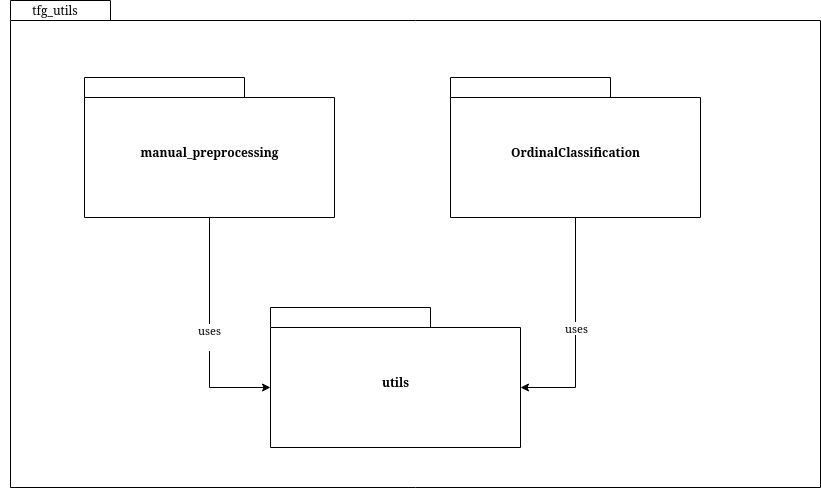
\includegraphics[scale=0.5]{diagrama_paquetes_tfg}
    \caption{Diagrama para paquete \textbf{tfg\_utils}}
    \label{dig:paquetes_tfg}
\end{figure}
En la Figura \ref{dig:paquetes_tfg} se muestra un gráfico que explica como se ha organizado el paquete de \textbf{tfg\_utils} que se ha desarrollado durante este trabajo.
\begin{itemize}
    \item \textbf{manual\_preprocessing} contiene una serie de funciones usadas en la fase de pre-procesamiento.
    \item \textbf{OrdinalClassification} contiene un paquete con la implementación del algoritmo de clasificación ordinal explicado en \ref{sec:ord}-\nameref{sec:ord}.
    \item \textbf{MultiLabelClassification} contiene un paquete con la implementación del algoritmo de clasificación muti-etiqueta ordinal que se ha propuesto en \ref{sec:cml}-\nameref{sec:cml}.
    \item \textbf{utils} contiene una serie de funciones que se han usado para todos los scripts. Contiene funciones para calcular las métricas, hacer la validación cruzada, etc.
\end{itemize}
A continuación se va a explicar las distintas clases que forman los paquetes \textbf{OrdinalClassification} y \textbf{MultiLabelClassification}. 
\clearpage
\subsection{Paquete para clasificación ordinal}
\label{sec:sftw-ocl}
A continuación se va a mostrar un diagrama explicando las clases que contiene el paquete \textbf{OrdinalClassification}:
\begin{figure}[H]
    \centering
    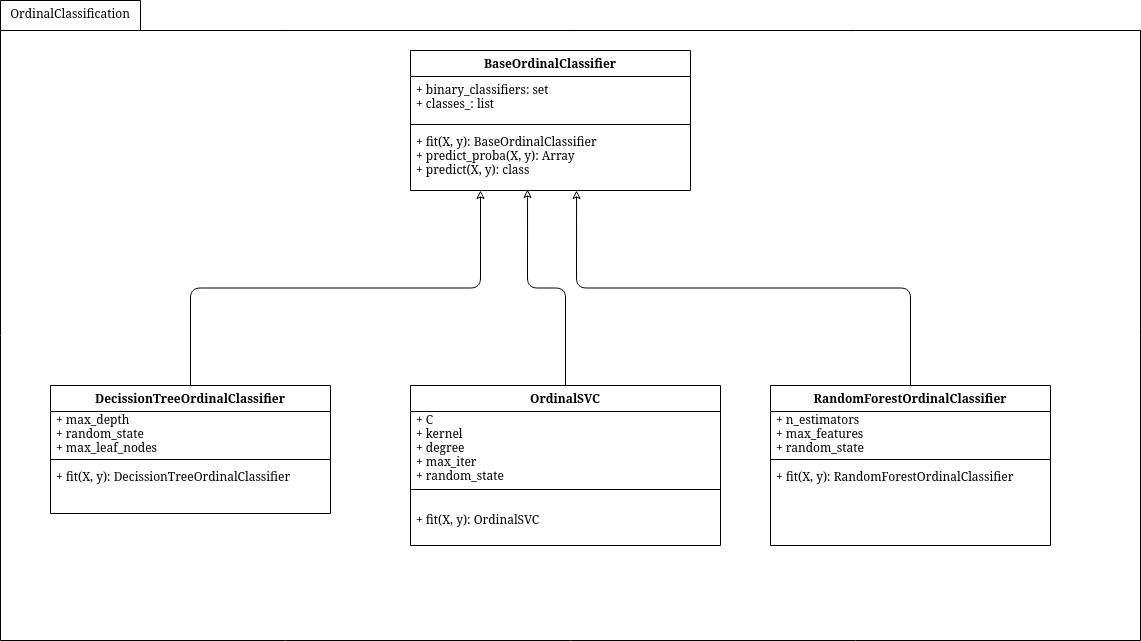
\includegraphics[scale=0.4]{diagrama_od}
    \caption{Diagrama para paquete \textbf{OrdinalClassification}}
    \label{dig:paquetes_od}
\end{figure}
En el diagrama mostrado en la Figura \ref{dig:paquetes_od}, se puede observar como existe una clase abstracta \textbf{BaseOrdinalClassifier} que contiene el algoritmo que se ha usado para realizar la clasificación ordinal de forma genérica. \\
Todas las clases que heredan de esta clase, especializan el algoritmo implementando en la clase base, usando un clasificador en especifico dependiendo del modelo que se quiera utilizar.\\
Dado que las funciones \textbf{\textit{predict}} (predice una clase dada una entrada) y \textbf{\textit{predict\_proba}} (dada una entrada predice la probabilidad de que una muestra pertenezca a cada clase) son iguales para todos los modelos, se ha optado por añadir estos métodos en la clase abstracta.\\
El resto de clases implementará el método \textbf{\textit{fit}} con el modelo seleccionado. \\
\linebreak
Cabe destacar que la implementación de estos modelos es compatible con todas las utilidades que proporciona \textit{scikit-learn}, ya que la clase base de donde están heredando las clases que implementan los modelos planteados (\textit{BaseOrdinalClassifier}) hereda a su vez de las clases \textit{ClassifierMixin} y \textit{BaseEstimator}, facilitando mucho el proceso de validación cruzada, optimización de parámetros y siguiendo la misma sintaxis que el resto de funcionalidades que proporciona \textit{scikit-learn}.
\subsection{Paquete para clasificación multi-etiqueta simple}
\label{sec:sftw-mlc}
Al igual que para crear las clases que implementan los modelos de clasificación ordinal, se ha seguido la misma metodología que la explicada previamente.\\
A continuación se muestra un diagrama explicando las clases que contiene el paquete \textbf{MultipleLabelClassification}:
\begin{figure}[H]
	\centering
	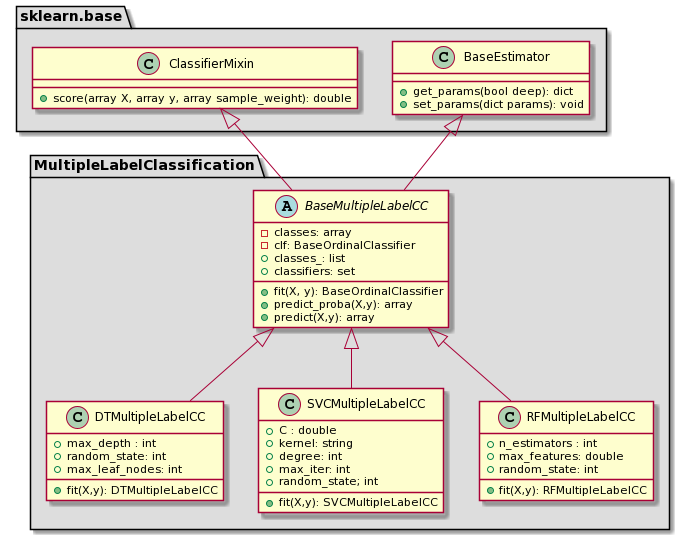
\includegraphics[scale=0.4]{diagrama_ml}
	\caption{Diagrama para paquete \textbf{MultipleLabelClassification}}
	\label{dig:paquetes_ml}
\end{figure}
Como se observa en la Figura \ref{dig:paquetes_ml}, se observa como se ha creado una clase abstracta (\textbf{BaseMultipleLabelCC}) que implementa el algoritmo que se ha usado de manera general y el resto de clases que heredan de esta, especializan la imlementación de ese algoritmo usando un clasificador distinto, dependiendo del modelo que se quiera usar.\\
\linebreak
Al igual que lo el paquete explicado en la Sección \ref{MultipleLabelClassification}, el que la clase base herede de las clases \textit{ClassifierMixin} y \textit{BaseEstimator} permite que las clases implementadas sean completamente compatibles con el resto de utilidades de \textit{Scikit-Learn}.
\section{Scripts}
Finalmente, la carpeta \textbf{\textit{scripts}} contiene todos los scripts usados para entrenar y mostrar resultados. Estos scripts son capaces de guardar la información obtenida en formato JSON y guardarlos en disco, facilitando así la integración con otras aplicaciones.\\
\linebreak
Se ha añadido también un script para comparar los resultados obtenidos por dos o más modelos, generando las gráficas que se han mostrado en secciones anteriores. Este script obtiene la información en formato JSON, especificando la ruta al archivo por linea de comandos. \\
\linebreak
Todos estos scripts, si se ejecutan con la opción \textbf{\textit{-h}} se mostrará una ayuda con todos los parámetros aceptados y una explicación de cada uno de ellos.
\section{Instalación del software}
Para instalar el software se necesita una versión 3.x de Python (durante el desarrollo se ha usado la versión 3.9.6) y el gestor de paquetes \textbf{pip}. Una vez descargado el repositorio(\href{https://github.com/antoniomanuelfr/TFG.git}{repositorio GitHub}), simplemente ejecutando el comando \textit{pip3 install .} en la carpeta padre del repositorio, se instalará el paquete junto con todas las dependencias.\\
A continuación, en la Figura \ref{cap:ex}, se muestra una captura de pantalla del proceso completo para ejecutar el algoritmo \nameref{alg:knn}:
\begin{figure}[H]
    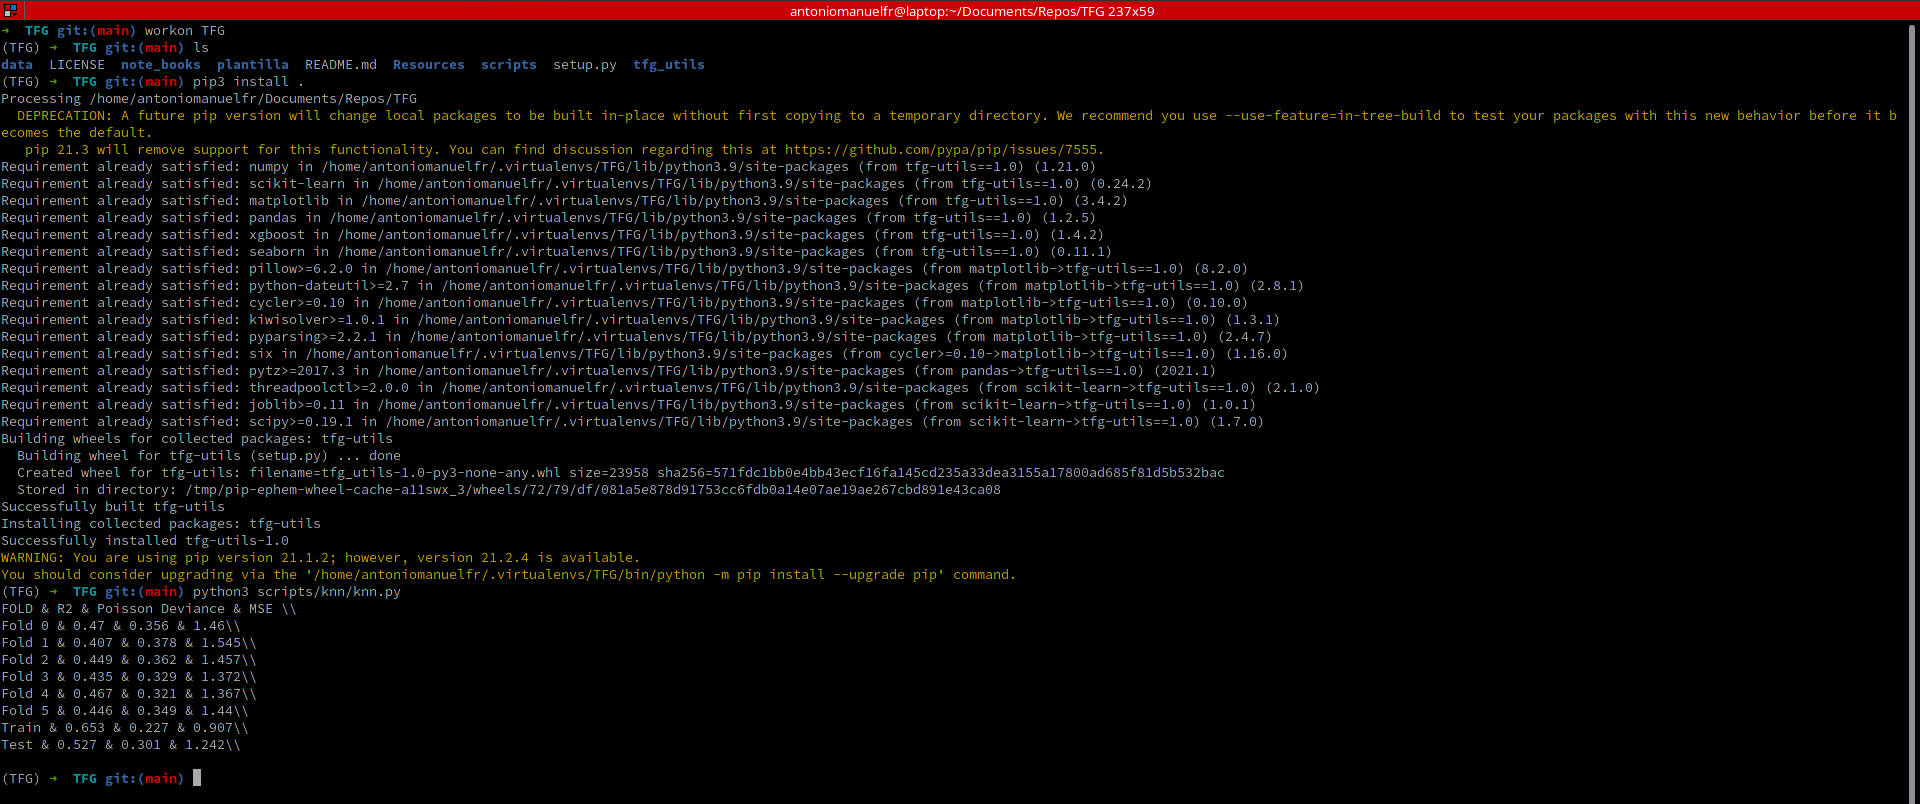
\includegraphics[scale=0.3]{ejemplo_ex}
    \caption{Ejemplo de ejecución completa para KNN}
    \label{cap:ex}
\end{figure}
En la Figura \ref{cap:ex} se observa como cuando se instala el paquete desarrollado, \textbf{pip} recupera todas las dependencias necesarias y se encarga de instalarlas previamente. \\
Una vez que se han instalado todas las dependencias necesarias, se puede ejecutar correctamente el script que ejecuta el modelo KNN para regresión sin ningún problema.\\
\linebreak
Aquí se muestra la principal ventaja de hacer uso de este tipo de paquetes que gestionan funciones comunes, ya que se facilita mucho la gestión de versiones y la gestión de dependencias.